\documentclass{standalone}

\usepackage{tikz}
% \usetikzlibrary{backgrounds}
% \usetikzlibrary{decorations.pathreplacing}

\renewcommand{\familydefault}{\sfdefault}

\begin{document}
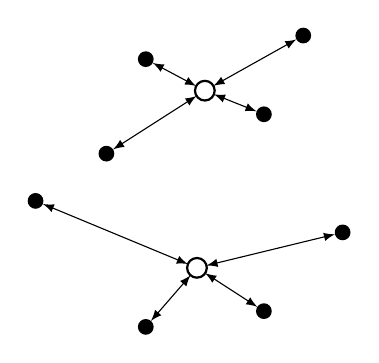
\begin{tikzpicture}
\tikzset{object/.style={fill,circle,minimum size=2mm,inner sep=0pt,outer sep=0mm}}
\tikzset{centroid/.style={draw,circle,thick,minimum size=2.5mm,inner sep=0pt,outer sep=0mm}}
\tikzset{a/.style={<->,>=latex}}

%\node at (0,0) {0};

%\node at (60:2)  [object] (0) {};
\node at (1,1.5) [object] (0) {};
%\node at (100:0.5)  [object] (1) {};
\node at (0.5,0.5) [object] (1) {};
%\node at (130:1.5)  [object] (2) {};
\node at (-1,1.2) [object] (2) {};
%\node at (180:1.5)  [object] (3) {};
\node at (-1.5,0) [object] (3) {};

\node at (-0.25,0.8) [centroid] (c0) {};

%\node at (200:3) [object] (4) {};
\node at (-2.4,-0.6) [object] (4) {};
%\node at (245:2.5) [object] (5) {};
\node at (-1,-2.2) [object] (5) {};
%\node at (285:2.2) [object] (6) {};
\node at (0.5,-2) [object] (6) {};
%\node at (330:2) [object] (7) {};
\node at (1.5,-1) [object] (7) {};

\node at (-0.35,-1.45) [centroid] (c1) {};

\draw [a] (c0) -- (0);
\draw [a] (c0) -- (1);
\draw [a] (c0) -- (2);
\draw [a] (c0) -- (3);

\draw [a] (c1) -- (4);
\draw [a] (c1) -- (5);
\draw [a] (c1) -- (6);
\draw [a] (c1) -- (7);

\end{tikzpicture}
\end{document}

